\documentclass[12pt]{article}
\usepackage[a4paper, total={6in, 8in}]{geometry}
\usepackage[utf8]{inputenc}
\usepackage{booktabs}
\usepackage{rotating}
\usepackage{multirow}
\usepackage[graphicx]{realboxes}
\usepackage{stackengine}
\usepackage{epigraph}
\usepackage{float}
\usepackage{dcolumn}
% \usepackage{longtable}
\usepackage{supertabular}
% \usepackage[nomarkers]{endfloat}
\usepackage{acronym}
\usepackage{listings}
\usepackage{hyperref}
\hypersetup{colorlinks=true,%
citecolor=black,%
filecolor=black,%
linkcolor=black,%
urlcolor=black
}
\usepackage[portuguese]{babel}
\usepackage[autostyle,portuguese=brazilian]{csquotes}
\usepackage{setspace} % for \onehalfspacing and \singlespacing macros
\onehalfspacing
\usepackage{etoolbox}
\usepackage{amsmath}
\AtBeginEnvironment{quote}{\singlespacing\small}
% \usepackage[usestackEOL]{stackengine}
\usepackage[justification=centering]{caption}
\usepackage[notes,backend=biber]{biblatex-chicago}
\usepackage{subfig} %incluir Figura side by side
%codigo  para spacing 1.5
%\usepackage{setspace}
%\doublespacing
%codigo para monospace justificado tt
\renewcommand{\familydefault}{\rmdefault}
%codigo estilo dos numeros
\usepackage[sc,osf]{mathpazo}
\usepackage{ragged2e}
\justifying

\usepackage{listings}
\usepackage{xcolor}

\definecolor{codegreen}{rgb}{0,0.6,0}
\definecolor{codegray}{rgb}{0.5,0.5,0.5}
\definecolor{codepurple}{rgb}{0.58,0,0.82}
\definecolor{backcolour}{rgb}{0.95,0.95,0.92}

\lstdefinestyle{mystyle}{
    backgroundcolor=\color{backcolour},   
    commentstyle=\color{codegreen},
    keywordstyle=\color{magenta},
    numberstyle=\tiny\color{codegray},
    stringstyle=\color{codepurple},
    basicstyle=\ttfamily\footnotesize,
    breakatwhitespace=false,         
    breaklines=true,                 
    captionpos=b,                    
    keepspaces=true,                 
    numbers=left,                    
    numbersep=5pt,                  
    showspaces=false,                
    showstringspaces=false,
    showtabs=false,                  
    tabsize=2
}

\lstset{style=mystyle}

\bibliography{references.bib}

\usepackage{enumitem}
\newlist{floatnotes}{description}{1}
\setlist[floatnotes]{font=\normalfont\itshape,wide, nosep, leftmargin=.1\linewidth, itemindent=\labelsep, rightmargin=\leftmargin, before=\vspace{.5em}\footnotesize}

\usepackage{pdflscape}
\usepackage{afterpage}
\usepackage{capt-of}% or use the larger `caption` package
\usepackage{enumitem}

\makeatletter
%Add packages here
\usepackage{hyperref}

\begin{document} 

\newgeometry{margin = .65in, top=1.05in}
\linespread{1.1}

\title{%
  A mulher negra no mercado de trabalho brasileiro: desigualdades salariais, representatividade e educação entre 2010 e 2022\\
  \vspace{1cm}
  \Large \texttt{\MakeUppercase{DRAFT}}}

\author{Pacto de Promoção da Equidade Racial \thanks{Responsáveis técnicos: Lucas Cavalcanti Rodrigues e Crislane Alves}}


\maketitle

\section{Introdução}

% Tendo em vista a amplitude do tema sob discussão, maior atenção será dada a dimensões previamente selecionadas, nomeadamente, desigualdades salariais, representatividade e educação.

\par Este texto de discussão tem como objetivo analisar as condições de participação da mulher negra no mercado de trabalho brasileiro no período compreendido entre os anos de 2010 e 2022. Em termos gerais, o presente estudo corrobora achados da literatura sobre o tema e indica novos achados que podem servir de base para investigações mais aprofundadas. No âmbito do diálogo com a literatura existente, o texto retoma fatos estilizados e traz dados atualizados que mostram que a mulher negra encontra-se em posição mais desfavorável no mercado de trabalho brasileiro, tanto em termos salariais quanto de representatividade, em relação aos demais subgrupos de\-mo\-grá\-fi\-cos sob análise \textemdash homens brancos, mulheres brancas e homens negros. Assim, mulheres negras recebem menores salários e, quando considerados recortes de sexo e cor da pele, respondem pelo menor percentual do total de trabalhadores empregados no mercado formal e informal de trabalho. 

\par Não obstante o quadro negativo observado, os dados indicam também que a representatividade da mulher negra no mercado de trabalho cresceu a taxas elevadas entre 2010 e 2020 no mercado formal. Este estudo sugere que, ao menos em parte, este forte aumento da participação da mulher negra deve-se ao rápido crescimento da escolaridade formal desse subgrupo demográfico no período. Com efeito, enquanto em 2010 apenas 13\% das mulheres negras no mercado formal de trabalho tinham ensino superior, em 2020 este percentual havia saltado para 20\%. Argumenta-se que esta mudança está possivelmente relacionada à polítca de cotas no ensino superior no período.


\par O presente documento divide-se em mais três seções, além dessa introdução. Na segunda seção discute-se aspectos mais gerais da participação da mulher negra no mercado de trabalho, usando-se os dados mais recentes da Pesquisa Nacional por Amostra de Domicílios Contínua (PNADC). Nesta seção, maior ênfase é dada a fatos estilizados documentados pela literatura. Na terceira seção, procura-se analisar as dimensões avaliadas na primeira seção em uma perspectiva temporal, com maior foco nas tendências observadas no mercado de trabalho formal. A última seção conclui o texto, resumindo os principais achados e indicando possíveis campos de ação para ampliação das melhorias observadas nos últimos anos, bem como caminhos para superação das limitações da participação da mulher negra no mercado de trabalho em áreas em que houve relativa estagnação nos últimos anos.

\section{Aspectos gerais e fatos estilizados} \label{overview}

\par Nesta seção, apresentam-se fatos estilizados sobre a participação da população negra no mercado de trabalho brasileiro, com ênfase no subgrupo demográfico representado pelas mulheres negras. Os fatos estilizados constituem-se em tendências conhecidas e documentadas na literatura existente sobre determinado tema de pesquisa.\footcite[178]{kaldor1961capital} Assim, guiando-se pela literatura existente, expõe-se nesta seção dados sobre diferenciais salariais, representativade e educação no mercado de trabalho brasileiro, considerando-se os recortes de sexo e cor da pele.

\par Considerando-se os diferenciais salariais, devem-se ser analisados quatro fatos estilizados sobre o tema sob análise, quais sejam, \textit{i)} Mulheres negras têm os menores salários médios quando se considera os quatro grupos formados por recorte de sexo e cor a pele; \textit{ii)} Desde 1987 observa-se uma convergência do nível salarial das mulheres negras em relação ao homem branco; \textit{iii)} As diferenças salariais nos 4 subgrupos de\-mo\-grá\-fi\-cos formados pela desagregação de sexo e cor da pele são maiores no Sudeste que no Nordeste; \textit{iv)} Existe um componente elitista nos diferenciais salariais de brancos e negros no mercado de trabalho brasileiro, ou seja, o salário relativo de negros diminui a medida que se avança na distribuição de rendimentos do trabalho.

\par O primeiro fato estilizado postula que, considerando os 4 subgrupos de\-mo\-grá\-fi\-cos sob análise, os salários médios das mulheres negras são os mais baixos, seguidos pelos salários de homens negros, mulheres brancas e homens brancos.\footcite{soares2000perfil,campante2004desigualdade} A literatura têm mostrado que essas desigualdades têm mudado ao longo do tempo, no sentido de diminuir a diferença salarial entre mulheres e homens. Soares (2000), por exemplo, mostra que entre 1987 e 1998, o \textit{gap} salarial entre mulheres negras e homens brancos diminuiu à taxa de 0,7\% ao ano. Enquanto para mulheres brancas essa redução foi de aproximadamente 1\% ao ano. Com efeito, em 1987, o rendimento médio mensal de mulheres negras representava 33\% do recebedido por homens brancos, enquanto em 1998 este percentual havia saltado para 40\%. Aparentemente, o ritmo de convergência diminuiu desde 1998, já que no segundo trimestre de 2022, dado mais recente da PNADC, o rendimento médio do trabalho da mulher negra passou a representar 46\% do ganho do homem branco (ver Figura \ref{fig:rendimento_trabalho}). 

\par A partir da observação da figura \ref{fig:rendimento_trabalho} também é possível observar uma outra característica do mercado de trabalho brasileiro quando se considera as clivagens de sexo e cor da pele, qual seja, a posição relativamente melhor da mulher negra em relação ao homem negro \textit{vis a vis} a mulher branca em relação ao homem branco. Nota-se, assim, que o rendimento da mulher negra é tipicamente 81,6\% do rendimento do homem negro, enquanto na comparação de mulheres brancas e homens brancos este rendimento é de 76,8\%.


\begin{figure}[H]
    \centering
    \caption{Rendimento médio do trabalho - Brasil - 2022}
        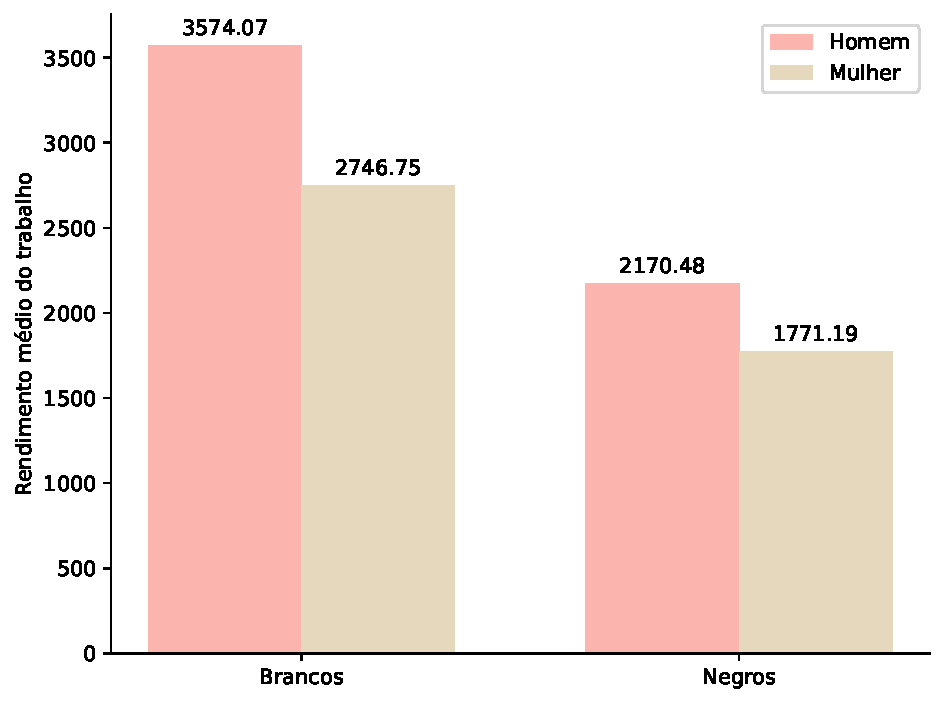
\includegraphics[height=8cm]{/home/dell/Documents/pacto/reports/black_women/figures/wage_2002_group.pdf}
    \label{fig:rendimento_trabalho}
    \begin{floatnotes}
        \item[Fonte:] Pesquisa Nacional por Amostra de Domicílios Contínua. 2º trimestre/2022.
        \item[Notas:] Para o cálculo, foram considerados apenas rendimento do trabalho de pessoas ocupadas com idade entre 14 e 65 anos.
    \end{floatnotes}
\end{figure}

\par Um outro fato estilizado é que as diferenças salariais nos subgrupos de\-mo\-grá\-fi\-cos analisados possui forte heterogeneidade regional.\footcite{campante2004desigualdade}. Neste sentido, o que a literatura tem mostrado é que as desigualdades salariais são muito mais pronunciadas no Nordeste do que no Sudeste. A Figura \ref{fig:rendimento_regiao} ilustra este fato. Fica claro que no Nordeste a discrepância salarial entre brancos e negros é muito maior que a diferença observada no Sudeste. Este efeito também aparece quando considera-se apenas as mulheres, já que no Nordeste a mulher negra recebe, em média, 71,2\% do rendimento de uma mulher branca, enquanto no Sudeste essa razão é de 62,4\% (ver Figura \ref{fig:rendimento_regiao_sexo}).


\begin{figure}[H]
    \centering
    \caption{Rendimento médio do trabalho - Sudeste e Nordeste - 2022}
        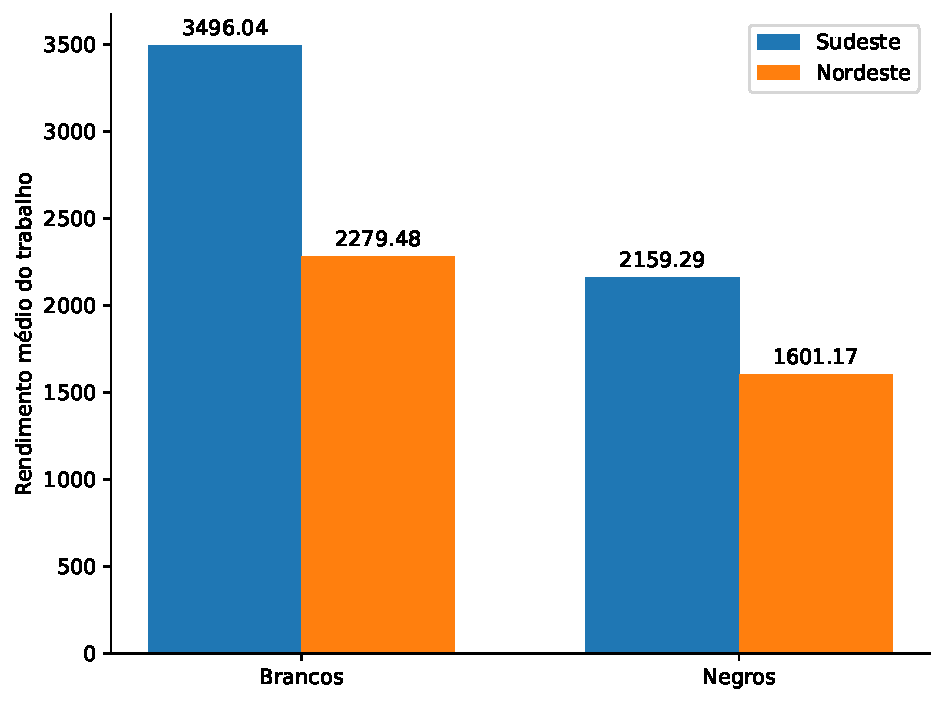
\includegraphics[height=8cm]{/home/dell/Documents/pacto/reports/black_women/figures/wage_2002_region.pdf}
    \label{fig:rendimento_regiao}
    \begin{floatnotes}
        \item[Fonte:] Pesquisa Nacional por Amostra de Domicílios Contínua. 2º trimestre/2022.
        \item[Notas:] Para o cálculo, foram considerados apenas rendimento do trabalho de pessoas ocupadas com idade entre 14 e 65 anos.
    \end{floatnotes}
\end{figure}

\begin{figure}[H]
    \centering
    \caption{Rendimento médio do trabalho de mulheres - Sudeste e Nordeste - 2022}
        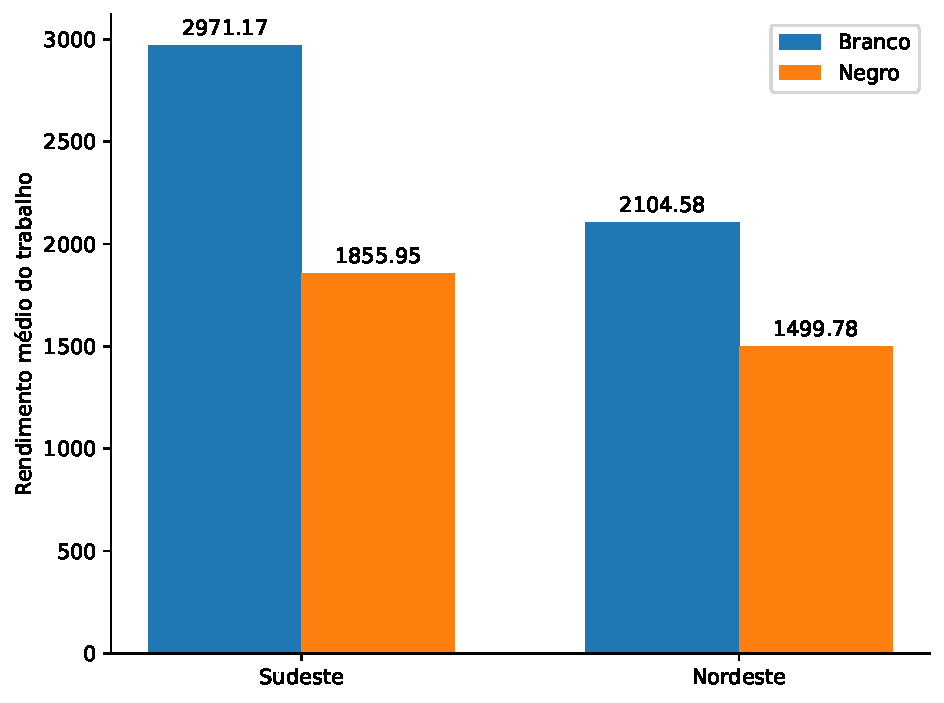
\includegraphics[height=8cm]{/home/dell/Documents/pacto/reports/black_women/figures/wage_2002_region_women.pdf}
    \label{fig:rendimento_regiao_sexo}
    \begin{floatnotes}
        \item[Fonte:] Pesquisa Nacional por Amostra de Domicílios Contínua. 2º trimestre/2022.
        \item[Notas:] Para o cálculo, foram considerados apenas rendimento do trabalho de pessoas ocupadas com idade entre 14 e 65 anos.
    \end{floatnotes}
\end{figure}

\par Uma fonte adicional de heterogeneidade nos diferenciais salariais entre brancos e negros é o nível de renda. Estudos mostram que quanto maior o nível do extrato de renda, maior é a parcela do diferencial de renda de brancos e negros que não é explicada por variáveis observadas. Esta característica dos diferenciais salariais por cor da pele no mercado de trabalho brasileiro é conhecida na literatura como \textit{discriminação elitista}.\footcite{soares2000perfil,campante2004desigualdade} Este fato é ilustrado pela Tabela \ref{tab:decis} que mostra o rendimento do trabalho para decis selecionados da distribuição de homens brancos, homens negros, mulheres brancas e mulheres negras. Para interpretar os resultados apresentados na tabela deve-se notar que os valores na células representam o montante recebido pelo indíviduo que divide a distribuição no ponto indicado. Por exemplo, a terceira linha da primeira coluna indica que 90\% dos homens brancos recebem até R\$ 7.500,00 por mês o que, reciprocamente, significa que esse é o valor mínimo dos 10\% de maior renda neste grupo.

\begin{table}[htb!]
    \centering
    \caption{Distribuição de rendimentos por sexo e cor - Brasil 2022}
    \begin{tabular}{lcccc}
    \hline
    Decil & \multicolumn{2}{c}{Brancos} & \multicolumn{2}{c}{Negros} \\ \cline{2-5} 
          & Homens      & Mulheres      & Homens      & Mulheres     \\ \hline
    10\%  & 1212        & 916           & 800         & 550          \\
    50\%  & 2000        & 1700          & 1500        & 1250         \\
    90\%  & 7500        & 5000          & 4000        & 3000         \\
    99\%  & 25000       & 17500         & 12000       & 9000         \\ \hline
    \end{tabular}
    \label{tab:decis}
    \begin{floatnotes}
      \item[Fonte:] Pesquisa Nacional por Amostra de Domicílios Contínua. 2º trimestre/2022.
      \item[Notas:] Para o cálculo, foram considerados apenas rendimento do trabalho de pessoas ocupadas com idade entre 14 e 65 anos.
  \end{floatnotes}
    \end{table}

\par Fica evidente, pela observação da Tabela \ref{tab:decis} que a diferença entre brancos e negros é maior nos decis e centis superiores da distribuição de rendimentos. Em particular, é possível notar que, entre os 10\% mais pobres, mulheres negras recebem pouco menos da metade do rendimento de homens brancos. E, entre o 1\% de maior renda, recebem cerca de 1/3 do rendimento de homens brancos. Essa tendência também pode ser observada para homens negros.

\par Os resultados acima indicam que mulheres negras encontram-se em posição desfavorável no mercado de trabalho quando consideramos os diferenciais salariais. O nível da desvantagem salarial da mulher negra, contudo, apresenta importantes heterogeneidades, a depender da região do país ou o extrato de renda considerados. Além disso, embora os resultados apresentem um quadro ruim, existem indicativos que a posição salarial da mulher negra tem tido uma melhoria relativa ao longo dos anos, com o salário médio de mulheres negras convergindo, ainda que lentamente, para os níveis observados para homens brancos. 

\par Os dados da distribuição de rendimentos do trabalho, contudo, explicam apenas parcialmente as condições de trabalho da mulher negra. Para que se observe um quadro mais amplo, é necessário levar em conta as taxas de participação e empregabilidade, considerando os recortes e de cor e sexo. Neste aspecto, os seguintes fatos estilizados devem ser mencionados: \textit{i)} mulheres negras formam o grupo com menor taxa de participação no mercado de trabalho; \textit{ii)} quando se considera a população empregada, mulheres negras são sobre-representadas no mercado informal de trabalho e em ocupações domésticas. Os dois fatos estilizados mencionados são ilustrados pelas figuras \ref{fig:employment} e \ref{fig:participation}.

\par A Figura \ref{fig:employment} mostra, para cada grupo de cor e sexo, o total de indíviduos desempregados e ocupados nos setores formal e informal. É possível notar que o desemprego e a informalidade é maior entre negros. Considerando-se a empregabilidade, os dados mostram que o desemprego nos quatro grupos sob análise foi de 11,1\% no segundo trimestre de 2022.\footnote{A taxa de desemprego calculada para os quatro grupos (11,1\%) difere da taxa de desemprego observada para economia como um todo (9,3\%) em função das diferenças de recortes demográficos e etários feitos para este estudo e os recortes utilizadas para o cômputo oficial da taxa de desemprego feita pelo IBGE} Essa média, porém, esconde elevada desigualdade entre os grupos. Com efeito, entre homens negros a taxa de desocupação foi de 10,1\% e, para mulheres negras, 17,1\% . No outro extremo da taxa de desemprego, encontram-se homens brancos, com 7,1\% de desocupação, enquanto mulheres brancas têm ocupação similar a de homens negros, 10,7\%.

\par Em relação à informalidade nota-se, novamente, dominância da população negra. Concretamente, no segundo trimestre de 2022, 53\% dos homens negros e 51,1\% das mulheres negras estavam no setor informal. Para a população branca esses percentuais foram, respectivamente, de 46,5\%  e 42\% . No entanto, assim como ocorre com os diferenciais salariais, a análise do quadro atual esconde a evolução observada nos últimos anos. Em particular, sabe-se que a participação da mulher negra no mercado formal de trabalho tem aumentado consistentemente recentemente. Como será visto na seção \ref{rais_representatividade}, dedicada ao estudo da representativade no setor formal, o número de mulheres negras com carteira assinada em relação ao de homens brancos avançou cerca de 20 pontos percentuais entre 2010 (30\%) e 2020 (50\%).

\begin{figure}[H]
    \centering
    \caption{Participação no mercado de trabalho - Brasil - 2022}
        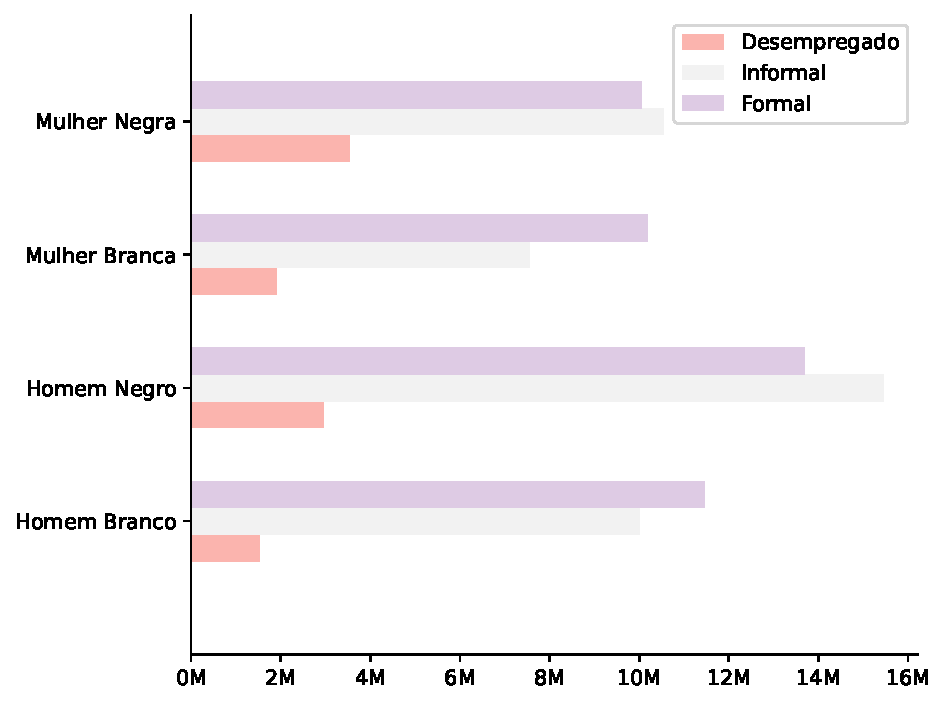
\includegraphics[height=8cm]{/home/dell/Documents/pacto/reports/black_women/figures/emprego.pdf}
    \label{fig:employment}
    \begin{floatnotes}
        \item[Fonte:] Pesquisa Nacional por Amostra de Domicílios Contínua. 2º trimestre/2022.
        \item[Notas:] Para o cálculo, foram considerados pessoas com idade entre 14 e 65 anos. Entre informais estão incluídos trabalhadores domésticos. Entre os ocupados, não foram considerados empregadores.
    \end{floatnotes}
\end{figure}


\begin{figure}[H]
    \centering
    \caption{Participação no mercado de trabalho - Setor Público e Privado - Brasil - 2022}
        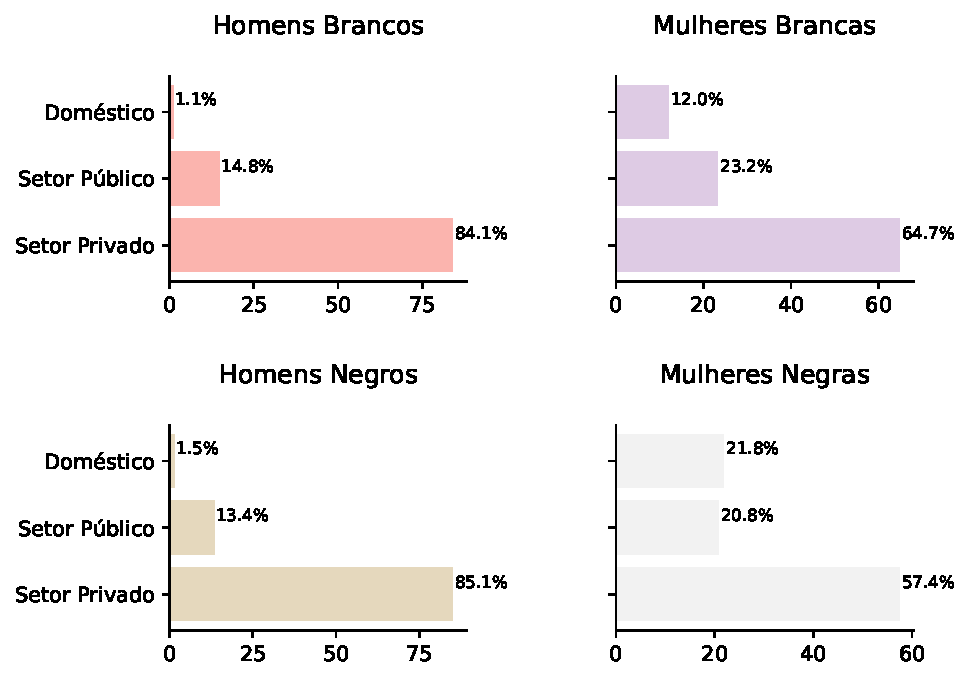
\includegraphics[height=8cm]{/home/dell/Documents/pacto/reports/black_women/figures/participation.pdf}
    \label{fig:participation}
    \begin{floatnotes}
        \item[Fonte:] Pesquisa Nacional por Amostra de Domicílios Contínua. 2º trimestre/2022.
        \item[Notas:] Para o cálculo, foram considerados apenas rendimento do trabalho de pessoas ocupadas com idade entre 14 e 65 anos.
    \end{floatnotes}
\end{figure}

\par Uma discussão importante foi levantada dentro da Teoria de Discriminação por Preferência de Becker (1957), de que quanto maior a competição no mercado de trabalho, menor será a discriminação com os empregados. Já que muitos empregadores têm preferências discriminatórias e esse efeito é naturalmente maior nas mulheres, em outras palavras, a contratação de uma mulher é uma desutilidade. Dessa forma, empregar uma mulher só terá utilidade se a dedução no salário compensar mais que proporcionalmente a perda da utilidade em contratá-la. Outros achados dentro dos Modelos de Discriminação Estátistica, corraboram com Becker, adicionando que, por antecipar que as mulheres deixaram o mercado de trabalho após terem filhos, algumas medidas acabam por exclui-las de incentivos à produtividade e garantia de permanência, ou seja, não é apenas a redução no salário.

\par No Brasil, talvez um dos principais direitos conquistados, dentro dessa vertente, promulgado na Constituição de 88 é a licença-maternidade, garantindo que, após o parto, a mulher, em regime de CLT, tenha um período de licença remunerada de 120 dias. Dentre os objetivos da licença-maternidade está a garantia de retornar ao trabalho após o fim da licença. No entanto, a literatura aponta que esse direito não é suficiente para a permanência da mulher no mercado formal, visto que as mulheres tendem a perder os empregos após terem filhos, mais especificamente após a licença-maternidade. 

\par O estudo de Machado (2016), traz evidências importantes, de que existe um aumento gradual da participação da mulher no mercado de trabalho formal até a licença-maternidade e, depois do período, há um declínio. A saída da mulher do mercado é motivada, quase sempre, por parte do empregador. 

\par A mesma autora aponta que, esses efeitos podem ser heterogêneos, variando de acordo, por exemplo, com o grau de escolaridade das mulheres, já que mulheres com maior nível de escolaridade apresentam queda de participação de 35\% após 12 meses do início da licença maternidade, e, do outro lado, mulheres com escolaridade mais baixa, o percentual é de 51\%. Evidências encontradas por Mattar (2018), mostram que após ter filhos a probabilidade da mulher ter um emprego não doméstico no setor formal diminui apenas para mulheres sem ensino superior.

\par Além do apresentado, o estudo citado apresenta também ações que podem ser somadas à licença-maternidade, por exemplo, a prorrogação. Foi encontrado resultados mais sólidos de proteção do emprego para mulheres que tiveram a licença prorrogada.

\par Outro ponto a se considerar é a natureza das ocupações, a literatura mais recente acerca da disparidade salarial de gênero, ressaltam a importância de se olhar para a demanda por flexibilidade no trabalho. Considerando que as mulheres possuem uma dupla jornada de laboral, quando somado o trabalho doméstico ao trabalho remunerado, empregos que demandam muitas horas e possuem horários inflexíveis, por exemplo, acabam sendo preteridos pelas mulheres uma vez que dificulta o equilíbrio entre o trabalho remunerado e doméstico. 

\par Sobre a demanda por flexibilidade, importante estudo de Mas e Pallais (2017), corrobora com a literatura relacionada a respeito do tema, de que as mulheres são mais inclinadas aos horários mais flexíveis de trabalho, mostrando que mulheres preferem trabalhar de casa, por exemplo em horário regulares. Por outro lado, as mulheres estão mais dispostas a empregos com maior estabilidade o que muitas vezes, assim como a flexibilidade, significa menor remuneração o que faz na verdade a mulher pagar por estabilidade e flexibilidade. 


\par De modo geral, é possível concluir que, tanto quando se considera os diferenciais salariais ou a participação no mercado de trabalho, a mulher negra encontra-se em desvantagem no mercado de trabalho. Há, contudo, evidências de que essas desvantagens podem estar diminuindo ao longo do tempo. Na seção seguinte, utiliza-se dados do mercado formal entre 2010 e 2020 e a metodologia do IEER para documentar com maior exatidão essas tendências.


\section{Representatividade e educação no mercado formal de trabalho} \label{rais_representatividade}

\par Na seção anterior, viu-se que mulheres negras encontram-se em posição desfavorável no mercado de trabalho quando consideramos os diferenciais salariais e taxas de participação. Notou-se também que o grau da desvantagem salarial varia, a depender da região do país ou o extrato de renda considerados. Em relação à participação no mercado de trabalho, notou-se que mulheres negras estão sobre-representadas entre não-ocupados, trabalhadores do setor informal e domésticas.
Além disso, embora os resultados apresentem um quadro ruim, existem indicativos que a posição da mulher negra no mercado de trabalho tem tido uma melhoria relativa ao longo dos anos, com o salário médio e as taxas de formalidade de mulheres negras convergindo, ainda que lentamente, para os níveis observados para homens brancos. Nesta seção, procura-se aprofundar a discussão sobre a evolução da participação da mulher negra no mercado de trabalho. Para isso, usa-se dados do mercado formal entre 2010 e 2020. Como ponto de partida para a discussão, usa-se o Índice ESG de Equidade Racial (IEER), métrica elaborada pelo Pacto pela Equidade Racial e utilizada por diversas empresas parceiras. Uma discussão completa sobre o IEER e suas propriedades pode ser encontrada no site Pacto. 

\par O primeiro resultado apresentado é o IEER atual das mulheres negras no mercado de trabalho formal brasileiro. Antes de apresentar os resultados, porém, é importante destacar uma questão relacionada à interpretação do IEER. O IEER, originalmente, mensura o número de desvios padrões em que o número de negros em determinada ocupação supera o valor esperado de negros dado uma população de referência. Esse valor, contudo, passa por uma transformação algébrica, com o objetivo de comparar o índice entre diferentes ocupações e empresas e fixar seu intervalo em [-1,1]. A transformação algébrica viabiliza a interpretação relativa, ao custo de limitar a possibilidade de interpretação absoluta do índice. Por essa razão, o valor do índice não pode ser interpretado em termos absolutos e, em particular, não tem uma interpretação de \enquote{elasticidade}. Um setor, por exemplo, com IEER=-0,32 não tem 32\% a menos de negros do que seria esperado. Esta é uma interpretação errada.

\par Por outro lado, a magnitude do valor absoluto do índice mostra sim \textit{o grau} de sub ou sobre-representação de negros na unidade produtiva. Assim, por exemplo, um empresa com IEER=-0.8 tem uma desigualdade racial nas suas ocupações \textit{maior} que uma empresa com IEER=-0.6. Para ajudar na interpretação dos valores do IEER, os autores do índice de equidade ocupacional, que serve de base para o IEER, sugeriram a seguinte classificação.\autocite{ransom2001one}

\begin{table}[htb!]
\centering
\caption{Interpretação dos intervalos do Índice ESG de Equidade Racial}
\begin{tabular}{lc}
\hline
Grupo             & Intervalo                 \\ \hline
Não-Mulher Negra Excluídos & $IEER \geq 0, 8 $               \\
Dominância Mulher Negra  & $0,2 < IEER < 0,8$   \\
Equidade          & $-0,2\leq IEER \leq 0,2$  \\
Dominância Não-Mulher Negra & $-0,8 < IEER < -0,2$ \\
Mulher Negra Excluída  & $IEER \leq -0,8$        \\ \hline
\end{tabular}
\end{table}

\par Os valores apresentados na Tabela \ref{tab:ieer_2020} mostram, então, que mulheres negras estão sub-representadas no mercado de trabalho formal brasileiro em uma proporção em que é possível falar em \textit{dominância} dos demais grupos de\-mo\-grá\-fi\-cos, mas não \textit{exclusão} de mulheres negras. Chega-se a essa interpretação ao se observar o valor do IEER Ponderado, principal indicador na Tabela \ref{tab:ieer_2020}. Os demais IEERs mostram a situação de representatividade de mulheres negras em 3 grupos de ocupação, não-liderança, gerência e diretoria. Fica claro que a representação de mulheres negras é maior em ocupações de não-liderança e diminui a medida que se avança no nível hierárquico das ocupações. Os resultados da Tabela \ref{tab:ieer_2020} referem-se a trabalhadores formais de todas as empresas brasileiras em 2020. É possível que os resultados observados variem quando se considera heterogeneidades regionais e econômicas das empresas.

\begin{table}[htb!]
    \centering
    \small
    \caption{Índice ESG de Equidade Racial - Mulheres Negras - 2020}
    \begin{tabular}{lc}
    \hline
    \multicolumn{1}{c}{Grupo} & IEER   \\ \hline
    Não-Liderança             & -0.579 \\
    Gerência                  & -0.656 \\
    Diretoria                 & -0.760 \\
    Ponderado                 & -0.665 \\ \hline
    \end{tabular}
    \label{tab:ieer_2020}
    \begin{floatnotes}
    \item [Fonte:] RAIS 2020.
    \item [Nota:] A população de referência utilizada é igual à metade da população de pretos e pardos.
    \end{floatnotes}
    \end{table}

\par Como a situação de representatividade da mulher negra de hoje se compara com a última década? Esta pergunta é respondida pela Figura \ref{fig:ieer_evolution} que apresenta a evolução do IEER Ponderado e dos IEERs ocupacionais de 2010 a 2020. Fica evidente que há uma evolução favorável no sentido de aumento da representação de mulheres negras nos últimos 10 anos. O resultado, que aparece no IEER Ponderado, é consequência da evolução favorável dos 3 IEERs ocupacionais, inclusive diretoria. Em que pese o fato da sub-representação de mulheres negras ser ainda muito elevada em 2020, como visto na Tabela \ref{tab:ieer_2020}.

\begin{figure}[H]
    \centering
    \caption{Evolução do IEER Ponderado - Mulheres Negras - 2010/2020}
        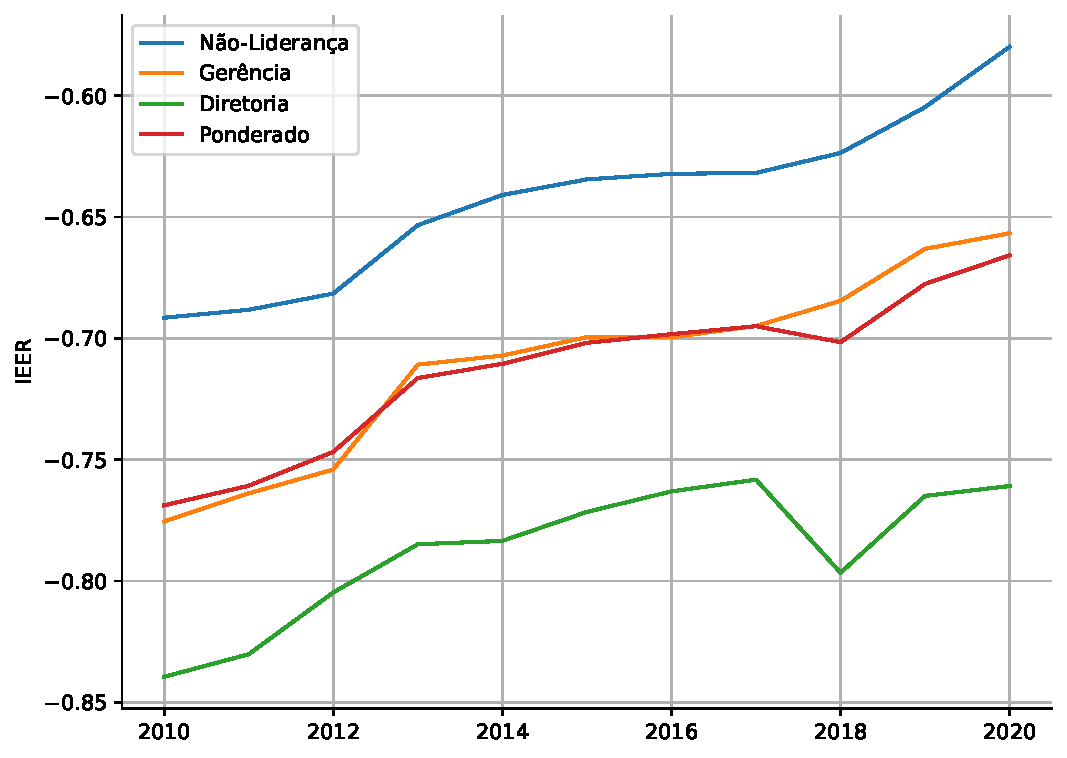
\includegraphics[height=8cm]{/home/dell/Documents/pacto/reports/black_women/figures/ieer_black_women.pdf}
    \label{fig:ieer_evolution}
\end{figure}

\par O IEER é uma medida de representatividade que leva em conta a desigualdade salarial. Isto porque o indicador de desigualdade ocupacional que serve de base para o IEER é ponderado pela massa salarial, dando maior peso a ocupações com maior nível salarial. Dessa forma, seria possível que parte da melhora observada na Figura \ref{fig:ieer_evolution} fosse causada pela queda da desigualdade salarial no período. A Figura \ref{fig:wage_gap} mostra, porém, que este não é o caso. Na figura, observa-se a evolução da proporção do salário de homens negros, mulheres brancas e mulheres negras em relação ao salário de homens brancos. Fica clara a lentidão da convergência salarial das mulheres negras no setor informal no período.

\begin{figure}[H]
    \centering
    \caption{Evolução do salário relativo em relação aos homens brancos - 2010/2020}
        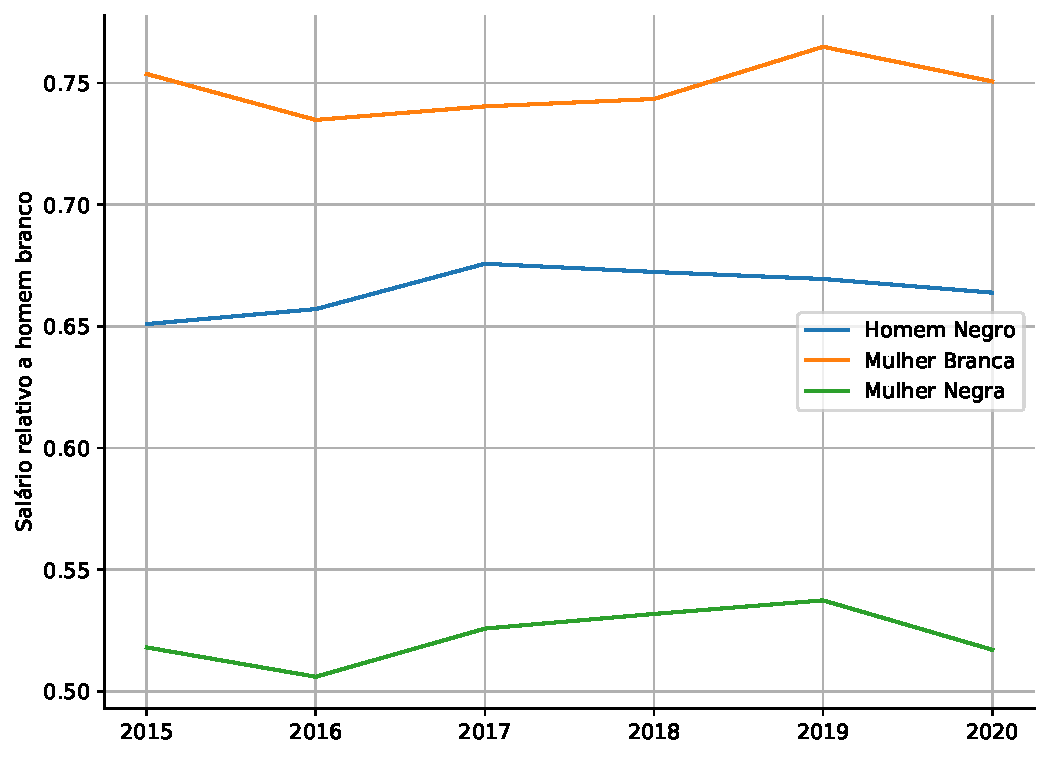
\includegraphics[height=8cm]{/home/dell/Documents/pacto/reports/black_women/figures/wage_gap.pdf}
    \label{fig:wage_gap}
\end{figure}

\par A Figura \ref{fig:supply_gap} mostra que, de fato, a provável explicação da melhora do IEER das mulheres negras na última década esteja no aumento do quantitativo de trabalhadores negros no mercado de trabalho formal no período. A Figura \ref{fig:supply_gap} mostra que, em relação a homens brancos, o número de mulheres negras com carteira assinada avançou cerca de 20 pontos percentuais, saindo de aproximadamente 30\% em 2010 e alcançando pouco mais de 50\% em 2020.


\begin{figure}[H]
    \centering
    \caption{Evolução da participação no mercado de trabalho formal em relação ao homem branco - 2010/2020}
        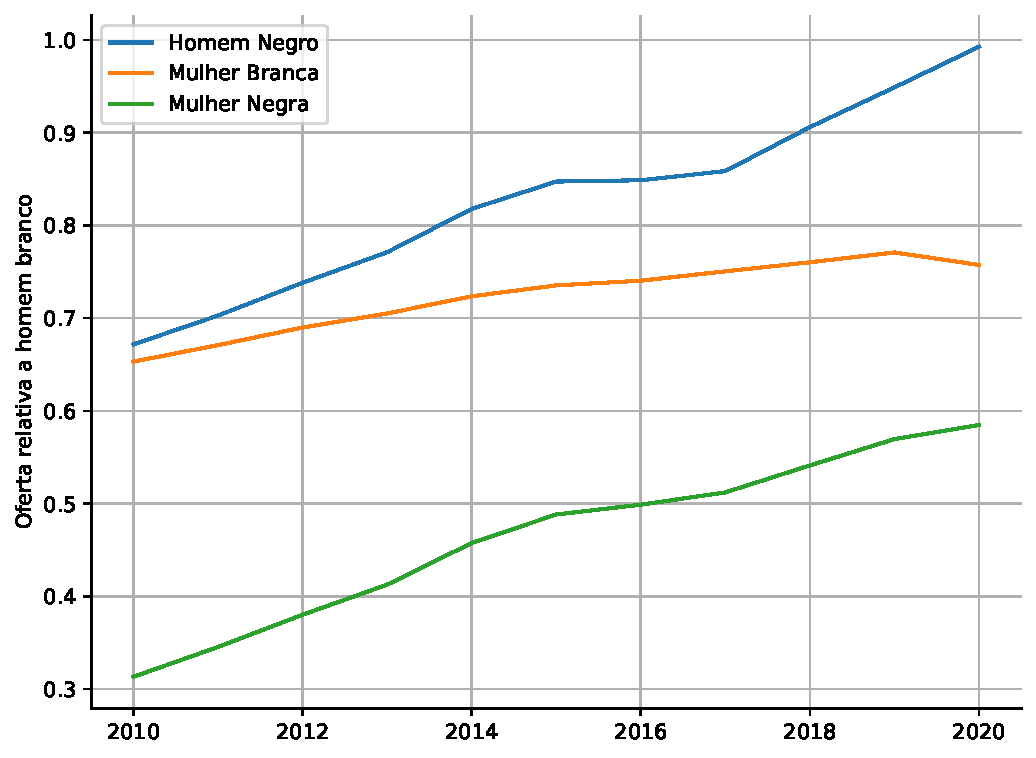
\includegraphics[height=8cm]{/home/dell/Documents/pacto/reports/black_women/figures/supply_gap.pdf}
    \label{fig:supply_gap}
\end{figure}

\par Uma provável explicação para as tendências observadas está na evolução da escolaridade da população negra no período. A Figura \ref{fig:rais_schooling} mostra que, entre trabalhadores ocupados no mercado formal, o total de trabalhadores com ensino superior entre homens negros saltou de 6\% para 10\%, enquanto para mulheres negras esse salto foi de 13\% para 21\%. Assim, é próvavel que por trás da relativa melhoria salarial e de participação laboral das mulheres negras observadas nas últimas décadas esteja o aumento da escolaridade da população negra no período.

% \begin{table}
\centering
\caption{Composição educacional da oferta de trabalho de mulheres negras - 2010-2020}
\begin{tabular}{lrrr}
\toprule
{} &  Até Fundamental &  Ensino Médio &  Superior+ \\
ano  &                  &               &            \\
\midrule
2010 &            23.9\% &         63.1\% &      13.0\% \\
2011 &            22.4\% &         64.5\% &      13.1\% \\
2012 &            21.3\% &         65.3\% &      13.4\% \\
2013 &            20.2\% &         65.9\% &      14.0\% \\
2014 &            18.5\% &         66.5\% &      15.0\% \\
2015 &            17.7\% &         66.6\% &      15.8\% \\
2016 &            16.3\% &         66.0\% &      17.7\% \\
2017 &            15.0\% &         66.3\% &      18.7\% \\
2018 &            14.0\% &         65.8\% &      20.1\% \\
2019 &            13.2\% &         66.4\% &      20.4\% \\
2020 &            12.4\% &         66.8\% &      20.8\% \\
\bottomrule
\end{tabular}
\end{table}

% \begin{table}[htb!]
\centering
\caption{Composição educacional da oferta de trabalho de homens negros - 2010-2020}
\begin{tabular}{lrrr}
\toprule
{} &  Até Fundamental &  Ensino Médio &  Superior+ \\
ano  &                  &               &            \\
\midrule
2010 &            45.8\% &         48.5\% &       5.7\% \\
2011 &            43.3\% &         50.8\% &       5.9\% \\
2012 &            40.9\% &         52.6\% &       6.5\% \\
2013 &            38.6\% &         54.6\% &       6.8\% \\
2014 &            36.1\% &         56.5\% &       7.5\% \\
2015 &            33.9\% &         58.3\% &       7.8\% \\
2016 &            31.5\% &         59.3\% &       9.2\% \\
2017 &            29.3\% &         61.2\% &       9.6\% \\
2018 &            28.0\% &         62.0\% &      10.0\% \\
2019 &            26.8\% &         63.2\% &      10.0\% \\
2020 &            25.7\% &         64.2\% &      10.1\% \\
\bottomrule
\end{tabular}
\end{table}


\begin{figure}[H]
    \centering
    \caption{Trabalhadores com ensino superior - População Negra - Brasil - 2022}
        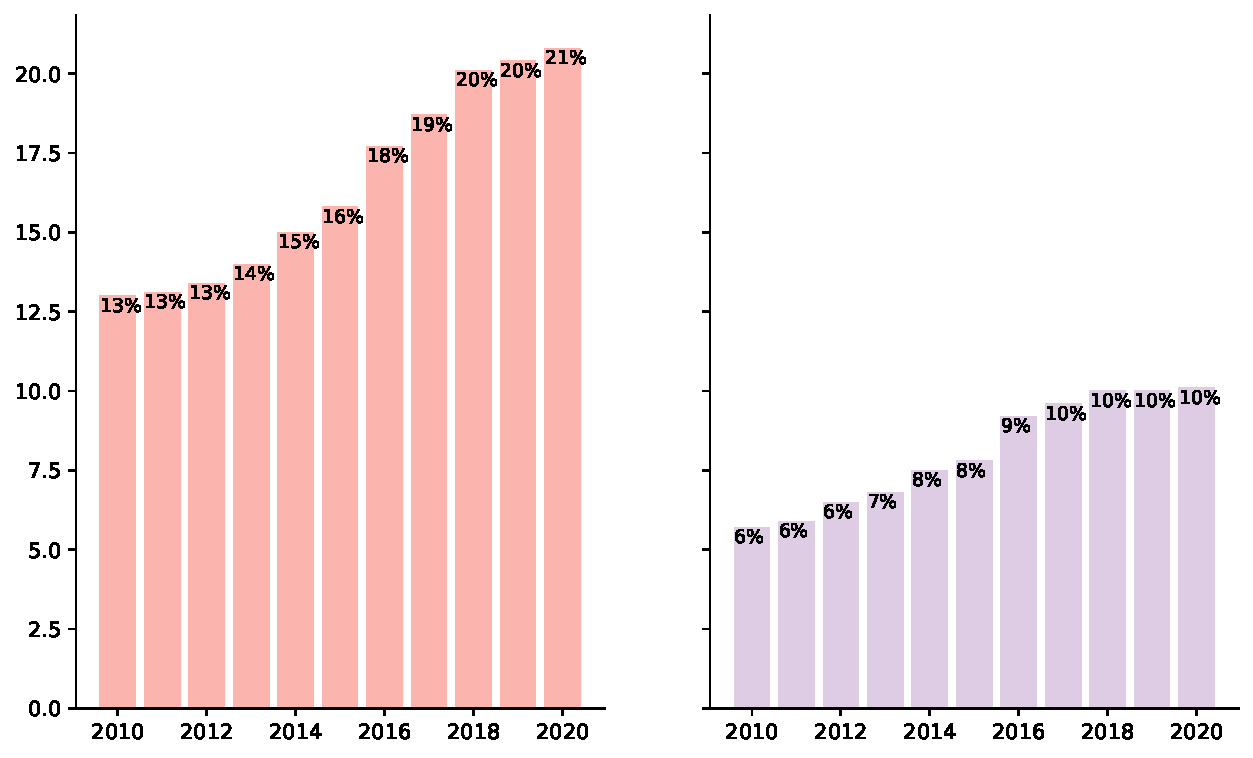
\includegraphics[height=8cm]{/home/dell/Documents/pacto/reports/black_women/figures/rais_schooling.pdf}
    \label{fig:rais_schooling}
    \begin{floatnotes}
        \item[Fonte:] RAIS 2010-2020.
        % \item[Notas:] Destaque dado a número de anos escolaridade que representam as etapas de ensino Fundamental, Médio e Superior.
    \end{floatnotes}
\end{figure}

\par O aumento da escolaridade da população negra nas últimas décadas é resultados de um ciclo virtuoso de políticas públicas implementadas desde a Constituição de 1988, onde incluem-se a ampliação do acesso à escola nos anos 1990 e as políticas afirmativas nas universidades desde o início dos anos 2000.\footnote{É possível, contudo, que o avanço na área de educação tenha beneficiado desproporciopnalmente mulheres negras, já que o racismo escolar, que pode causar retenção e abandono, afeta mais frequentemente homens negros (Ver \autocite{carvalho2004fracasso}). As figuras \ref{fig:white_schooling} e \ref{fig:black_schooling}, em anexo, mostram que mulheres têm \textit{achievement} escolar consistentemente maiores que homens, mas essa diferença é mais pronunciada e manifesta-se mais cedo ao longo da vida escolar entre negros.}

\par Alguns estudos argumentam, contudo, que parte relevante do aumento da taxa de ensino superior entre mulheres negras concentrou-se em IESs privadas e cursos de menor prestígio.\footcite[Cap. 1]{marcondes2013dossie} A participação maior de mulheres negras em cursos de ensino superior de menor prestígio pode reduzir a probabilidade \textit{matching} entre área de formação e área de atuação, além de aumentar a probabilidade de mulheres negras serem alocadas em setores de menor prêmio salarial. A Tabela \ref{tab:sup_setor}, que traz dados da distribuição de trabalhadores com ensino superior nos 5 setores de menor remuneração na economia em 2020, parece corroborar este fato. Os dados na tabela indicam que cerca de 45\% das mulheres negras com ensino superior trabalham nos 5 setores de pior remuneração na economia. Em contrapartida, apenas 25\% dos homens brancos com ensino superior estão alocados nestes setores. A hierarquia dos grupos se inverte quando se considera os 5 setores de maior remuneração, como pode ser visto na Tabela \ref{tab:sup_setor_high}



\begin{table}[htb!]
    \centering
    \small
    \caption{Distribuição de trabalhadores com ensino superior por setor \\ 5 setores de menor remuneração - 2020}
    \begin{tabular}{lcccc}
        \hline
        \multicolumn{1}{c}{\multirow{2}{*}{Subsetor}}                                                               & \multicolumn{2}{c}{Homens}                               & \multicolumn{2}{c}{Mulheres}                             \\
        \multicolumn{1}{c}{}                                                                                        & \multicolumn{1}{r}{Brancos} & \multicolumn{1}{r}{Negros} & \multicolumn{1}{r}{Brancas} & \multicolumn{1}{r}{Negras} \\ \hline
        Indústria têxtil do vestuário e artefatos de tecidos                                                        & 0.6                         & 0.4                        & 0.8                         & 0.5                        \\
        \begin{tabular}[c]{@{}l@{}}Serv. de alojamento, alimentaçao, \\ reparaçao, manutençao, redaçao\end{tabular} & 5.6                         & 7.1                        & 8.0                         & 9.3                        \\
        Comércio varejista                                                                                          & 7.2                         & 8.7                        & 8.6                         & 9.9                        \\
        Administraçao pública direta e autárquica                                                                   & 3.7                         & 4.0                        & 8.3                         & 7.9                        \\
        Ensino                                                                                                      & 10.8                        & 11.0                       & 17.2                        & 17.3                       \\ \hline
        \end{tabular}
    \label{tab:sup_setor}
    \begin{floatnotes}
        \item [Fonte:] RAIS 2020.
        % \item [Nota:] 
        \end{floatnotes}
    \end{table}


\begin{table}[htb!]
    \centering
    \small
    \caption{Distribuição de trabalhadores com ensino superior por setor \\ 5 setores de maior remuneração - 2020}
    \begin{tabular}{lcccc}
        \hline
        \multicolumn{1}{c}{\multirow{2}{*}{Subsetor}}                                                               & \multicolumn{2}{c}{Homens}                               & \multicolumn{2}{c}{Mulheres}                             \\
        \multicolumn{1}{c}{}                                                                                        & \multicolumn{1}{r}{Brancos} & \multicolumn{1}{r}{Negros} & \multicolumn{1}{r}{Brancas} & \multicolumn{1}{r}{Negras} \\ \hline
        Extrativa mineral                                                                                           & 0.9                         & 1.4                        & 0.3                         & 0.4                        \\
        Serviços industriais de utilidade pública                                                                   & 2.0                         & 1.8                        & 0.8                         & 0.7                        \\
        \begin{tabular}[c]{@{}l@{}}Ind. química de produtos farmacêuticos, \\ veterinários, perfumaria\end{tabular} & 3.7                         & 2.6                        & 2.3                         & 1.4                        \\
        Indústria do material de transporte                                                                         & 2.6                         & 1.1                        & 0.7                         & 0.3                        \\
        Instituiçoes de crédito, seguros e capitalizaçao                                                            & 10.4                        & 7.2                        & 9.2                         & 5.7                        \\ \hline
        \end{tabular}
    \label{tab:sup_setor_high}
    \begin{floatnotes}
        \item [Fonte:] RAIS 2020.
        % \item [Nota:] 
        \end{floatnotes}
    \end{table}

\par Essa tendência pode explicar o fato da convergência salarial ser muito menos pronunciada que a tendência observada nas taxas de participação. Assim, é possível que o aprofundamento e aceleração das melhorias das condições de trabalho da mulher negra passe pela continuidade do avanço na escolaridade, bem como o aumento da qualidade da inserção da mulher negra no ensino superior e nos setores de maior remuneração na economia.

\section{Conclusão}

\par O propósito do presente estudo foi analisar e discutir a participação da mulher negra no mercado de trabalho nos últimos doze anos. O que se verificou, a partir da literatura revisada e da exploração dos dados, é que de fato existe uma diferença negativa no posicionamento da mulher negra no mercado de trabalho brasileiro, tanto em termos de alocação, quanto em termos salariais e esta desigualdade pode ser encontrada no mercado formal e informal.
\par Com o objetivo de fornecer um senso comparativo para a análise, foram usados 4 subgrupos demográficos, a saber: mulheres negras, homens negros, mulheres brancas e homens brancos. Assim, foi possível localizar o estudo em dois eixos principais: sexo e cor da pele. Portanto, considerando tal divisão, verificou-se que, no mercado nacional, mulheres negras têm salários médios inferiores aos de homens negros e brancos, e de mulheres brancas. Por outro lado, um fator anexo dentro desta análise é que, ainda considerando as desagregações por sexo e cor da pele, para o ano de 2022, a mulher negra tem um \textit{gap} de rendimento médio menor com relação ao homem negro, do que a mulher branca acerca do homem branco. 
\par Outra ótica analisada foi a regional e foi possível observar grande heterogeneidade. A exploração de dados, para o segundo trimestre de 2022, mostra que trabalhadores negros no Nordeste receberam, em média, de 70\% do rendimento de trabalhadores brancos. No Sudeste o trabalhador negro tem, em média, 62\% do ganho do trabalhador branco. Quando se trata do recorte feminino para o mesmo período de análise, essa lógica se mantém, já que a mulher negra recebe 71\% do rendimento médio de uma mulher branca no Nordeste. No Sudeste a diferença é de 62\%.
\par Adicionalmente, analisou-se o diferencial salarial de brancos e negros sob a perspectiva do nível de renda para o 2022 do mercado de trabalho brasileiro. Aqui, constatou-se que esse diferencial é maior quanto maior for o nível de extrato da renda. Quando se tratando de mulheres negras, observou-se que nos 10\% mais pobres, as mulheres recebem menos que a metade do ganho salarial de homens brancos e, entre o 1\% mais ricos, cerca de 1/3. Apesar da desvantagem assinalada, ao longo dos anos a posição salarial da mulher negra, com relação aos homens brancos, mesmo que lentamente, vem melhorando.
\par Para ampliar o estudo também foram observadas as taxas de participação e empregabilidade da mulher negra no mercado de trabalho formal e informal. Assim, foi constatado que mulheres negras possuem a menor taxa de participação no mercado de trabalho e, ainda, uma sobre-representação no mercado informal e em ocupações domésticas. No entanto, a participação da mulher negra no mercado formal de trabalho tem aumentado nos últimos anos. A título de comparação, o número de mulheres negras com carteira assinada em relação ao de homens brancos avançou cerca de 20 pontos percentuais entre 2010 e 2020, por exemplo.
\par No que tange a evolução da mulher negra no mercado de trabalho brasileiro, foi utilizado o Índice ESG de Equidade Racial (IEER), que leva em conta a desigualdade salarial, com objetivo de aprofundar a discussão. Os resultados apontam que, para o mercado formal em 2020,  apesar de não existir exclusão de mulheres negras, essas estão sub-representadas, e, ainda, revela uma dominância dos demais subgrupos demográficos. Ainda, é possível notar que a representação de mulheres negras é maior em ocupações de não liderança e, do lado oposto, quanto maior o nível hierárquico das ocupações, como cargos de liderança e diretoria, a partição tende a diminuir. Fazendo comparativo com a década anterior, o valor ponderado do índice em 2010 era de (-0.77) e em 2020 foi de (-0.67), o que demonstra que, apesar dos resultados negativos,  há indícios de uma evolução favorável. \par Existem indicativos de que essa crescente melhora salarial e da participação das mulheres negras no mercado nos últimos 10 anos possa ser explicada pelo aumento da escolaridade da população negra no período que, por sua vez, é fruto de políticas públicas que incluíam, dentre  outras coisas, a ampliação do acesso à escola e políticas de cota, por exemplo. Não obstante, a literatura aponta que essa partição reteve-se em instituições de ensino privadas e cursos considerados de menor prestígio. A consequência disso é que pode reduzir a probabilidade de \textit{matching} entre área de formação e área de atuação, além de aumentar a probabilidade de mulheres negras serem alocadas em setores de menor prêmio salarial.
\par Desse modo, tanto a literatura revisada quanto a exploração dos dados utilizados nesta discussão confirmam que, ao se considerar diferenças salariais e taxas de participação, as mulheres negras estão em posição desfavorável no mercado de trabalho brasileiro para o recorte analisado, mesmo considerando algumas regiões do país e o extrato de rendimento. Notou-se também que, apesar dos resultados negativos, existem evidências de melhora desses indicadores ao longo dos anos. Para estudos futuros, pretende-se adicionar a essa discussão a inclusão de anos de escolaridade da população negra e branca, ampliar o recorte regional para outros países, além de aumentar a literatura utilizada.

\clearpage

\appendix

\section*{Figuras Complementares} \label{fig_comp}

\begin{figure}[H]
    \centering
    \caption{Anos de escolaridade - População Branca - Brasil - 2022}
        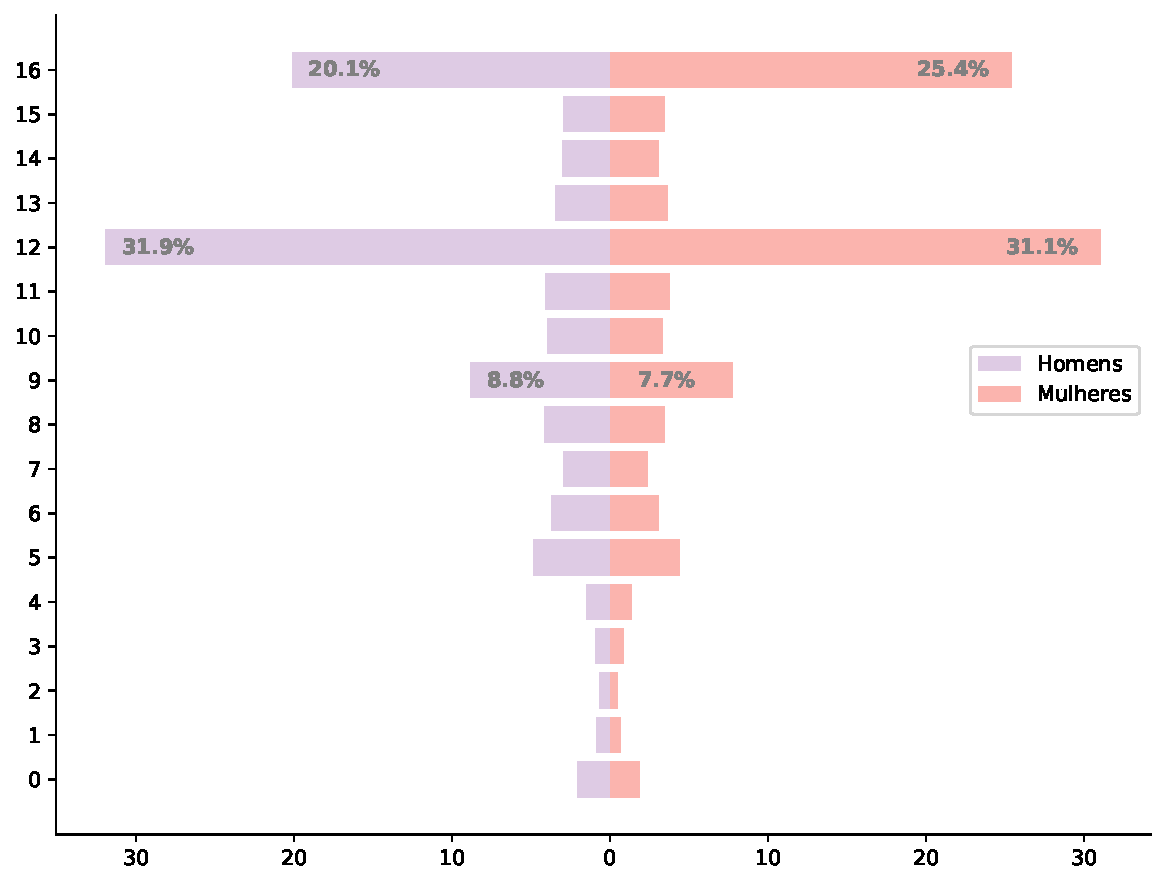
\includegraphics[height=8cm]{/home/dell/Documents/pacto/reports/black_women/figures/schooling_white.pdf}
    \label{fig:white_schooling}
    \begin{floatnotes}
        \item[Fonte:] Pesquisa Nacional por Amostra de Domicílios Contínua. 2º trimestre/2022.
        \item[Notas:] Destaque dado a número de anos escolaridade que representam as etapas de ensino Fundamental, Médio e Superior.
    \end{floatnotes}
\end{figure}

\begin{figure}[H]
    \centering
    \caption{Anos de escolaridade - População Negra - Brasil - 2022}
        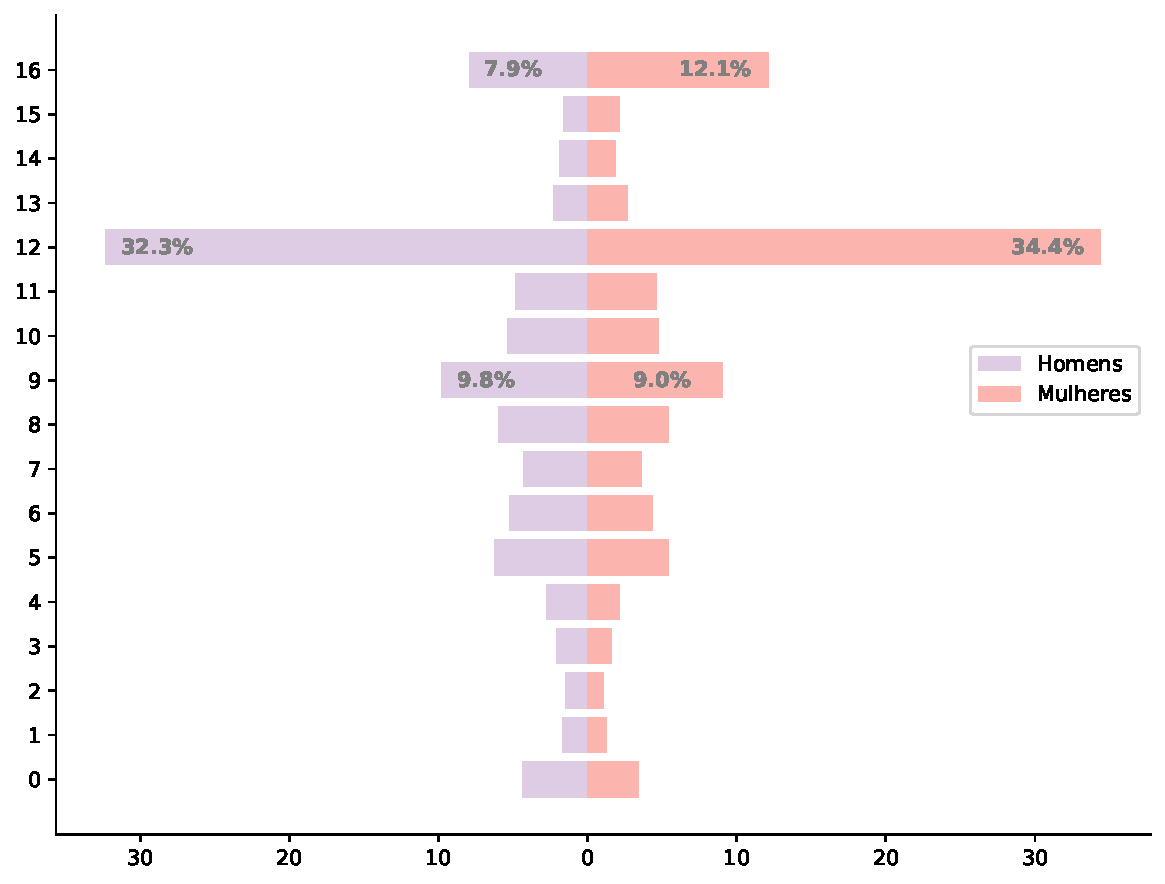
\includegraphics[height=8cm]{/home/dell/Documents/pacto/reports/black_women/figures/schooling_black.pdf}
    \label{fig:black_schooling}
    \begin{floatnotes}
        \item[Fonte:] Pesquisa Nacional por Amostra de Domicílios Contínua. 2º trimestre/2022.
        \item[Notas:] Destaque dado a número de anos escolaridade que representam as etapas de ensino Fundamental, Médio e Superior.
    \end{floatnotes}
\end{figure}

\printbibliography[title={Bibliografia}, nottype=misc]



\end{document}